\subsection{Caso d'uso UC9: Modifica della presentazione}
\begin{figure}[h] 
	\centering 
	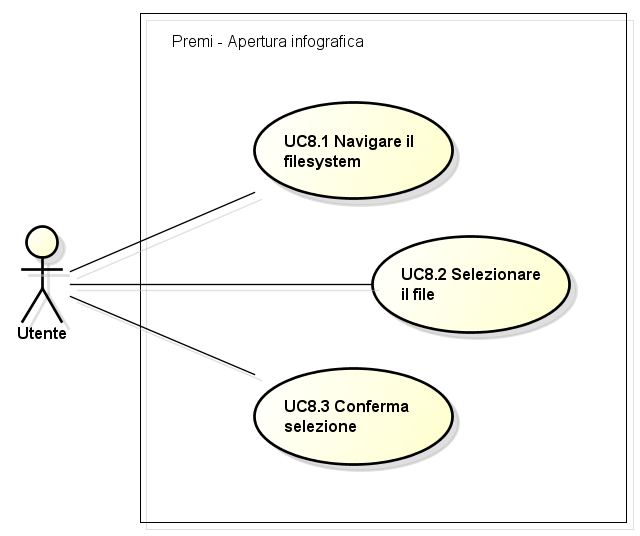
\includegraphics[scale=0.35] {img/UC9.png} 
	\caption{UC9 - Modifica della presentazione} 
\end{figure}

\begin{itemize}
	\item \textbf{Attori:} Proprietario;
	\item \textbf{Scopo e descrizione:} L'utente sta lavorando su una presentazione per inserire delle nuove \gls{slide} o per modificare quelle già create. Può quindi inserire  elementi come: \gls{slide}, immagini, caselle di testo, dati \gls{real time}. Ha inoltre la possibilità di modificare gli elementi già inseriti, oppure di eliminarli. Può infine scegliere l'effetto di transizione tra una \gls{slide} e l'altra;
	\item \textbf{Precondizione:} L'utente ha creato una presentazione nella fase di creazione di un progetto;
	\item \textbf{Flusso principale degli eventi:}
	\begin{enumerate}
		
		\item L'utente sceglie il \gls{template} [UC9.1];
		
		\item L'utente inserisce una nuova \gls{slide} [UC9.2];
		\item L'utente rimuove una \gls{slide} [UC9.3];
		
		\item L'utente inserisce un'immagine [UC9.4];
		
		\item L'utente inserisce una casella di testo [UC9.5];
		
		\item L'utente inserisce dati \gls{real time} [UC9.6];
		
		\item L'utente inserisce una tabella [UC9.7];
		
		\item L'utente inserisce un grafico [UC9.8];
		
		\item L'utente sceglie un effetto di transizione [UC9.9];
		
		\item L'utente cambia la dimensione di un elemento [UC9.10];
		
		\item L'utente cambia la posizione di un elemento [UC9.11];
		
		\item L'utente ruota un elemento [UC9.12];
		
		\item L'utente rimuove un elemento [UC9.13];
		
		\item L'utente carica un file per inserire l'immagine [UC9.14];
		\item L'utente sceglie la formattazione del testo [UC9.15];
		\item L'utente modifica una tabella [UC9.16];
		\item L'utente modifica un grafico [UC9.17];
		
		\item L'utente inserisce note/parole chiave [UC9.18].
	\end{enumerate}
	\item \textbf{Postcondizione:} Il sistema esegue le operazioni effettuate dall'utente.
\end{itemize}


\subsection{Caso d'uso UC9.1: Scegliere un \gls{template}}
\begin{itemize}
	\item \textbf{Attori:} Proprietario;
	\item \textbf{Scopo e descrizione:} L'utente sceglie un \gls{template} di stile da utilizzare per la propria presentazione;
	\item \textbf{Precondizione:} Il sistema è in attesa che l'utente selezioni il \gls{template} da utilizzare;
	\item \textbf{Postcondizione:} Il sistema imposta il \gls{template} selezionato per la presentazione.
\end{itemize}


\subsection{Caso d'uso UC9.2: Inserire una nuova \gls{slide}}
\begin{itemize}
	\item \textbf{Attori:} Proprietario;
	\item \textbf{Scopo e descrizione:} L'utente crea una nuova \gls{slide} nella presentazione per poter inserire del contenuto;
	\item \textbf{Precondizione:} Il sistema è in attesa che l'utente crei una nuova \gls{slide};
	\item \textbf{Postcondizione:} Il sistema ha creato la nuova \gls{slide}.
\end{itemize}


\subsection{Caso d'uso UC9.3: Rimuovere una \gls{slide}}
\begin{itemize}
	\item \textbf{Attori:} Proprietario;
	\item \textbf{Scopo e descrizione:} L'utente vuole rimuovere una \gls{slide} della presentazione precedentemente creata;
	\item \textbf{Precondizione:} Il sistema è in attesa che l'utente selezioni una \gls{slide} e il comando per rimuoverla;
	\item \textbf{Postcondizione:} Il sistema ha rimosso la \gls{slide} selezionata.
\end{itemize}


\subsection{Caso d'uso UC9.4: Inserire un'immagine}
\begin{itemize}
\item \textbf{Attori:} Proprietario;
\item \textbf{Scopo e descrizione:} L'utente deve inserire un'immagine in una \gls{slide}. Seleziona il comando e sceglie l'immagine da inserire nella \gls{slide} corrente;
\item \textbf{Precondizione:} Il sistema è in attesa che l'utente selezioni il comando per inserire un'immagine;
\item \textbf{Postcondizione:} Il sistema ha inserito l'immagine selezionata dall'utente nella \gls{slide}.
\end{itemize}


\subsection{Caso d'uso UC9.5: Inserire una casella di testo}
\begin{itemize}
\item \textbf{Attori:} Proprietario;
\item \textbf{Scopo e descrizione:} L'utente deve inserire una casella di testo nella \gls{slide}. Seleziona il comando e inserisce la casella di testo nel punto della \gls{slide} desiderato;
\item \textbf{Precondizione:} Il sistema è in attesa che l'utente selezioni il comando per inserire una casella di testo;
\item \textbf{Postcondizione:} Il sistema ha inserito la casella di testo nella \gls{slide}.
\end{itemize}


\subsection{Caso d'uso UC9.6: Inserire dati real time}
\begin{itemize}
	\item \textbf{Attori:} Proprietario;
	\item \textbf{Scopo e descrizione:}	L'inserimento di un dato \gls{real time} consiste nell'inserimento di una stringa speciale che si occuperà di richiamare dei contenuti personalizzabili definiti precedentemente dall'utente. Questi contenuti hanno il compito di catturare dati provenienti dall'esterno per poi riportarli nelle \gls{slide} ed avere così dati aggiornati in tempo reale in quanto saranno composti di codice eseguito a run-time dal server. Nel caso la presentazione venga visualizzata offline, i contenuti faranno riferimento ai dati ottenuti nel momento dell'inserimento dell'oggetto.
	L'utente, quindi, deve inserire dei dati \gls{real time}. Per inserirli deve caricare prima il codice che vuole richiamare attraverso l'oggetto inserito, poi inserire l'oggetto all'interno della presentazione indicando la funzione che deve svolgere.
	
	\item \textbf{Precondizione:} Il sistema è in attesa che l'utente inserisca i dati \gls{real time};
	\item \textbf{Flusso principale di eventi:}
	\begin{enumerate}
		\item L'utente inserisce il file contenente il codice da eseguire [UC9.6.1].
	\end{enumerate}
	\item \textbf{Postcondizione:} Il sistema ha inserito i dati \gls{real time}.
\end{itemize}

	\subsection{Caso d'uso UC9.6.1: Inserire un file di codice}
	\begin{itemize}
		\item \textbf{Attori:} Proprietario;
		\item \textbf{Scopo e descrizione:} L'utente deve inserire un file di codice da usare per un oggetto di dati \gls{real time};
		\item \textbf{Precondizione:} Il sistema è in attesa che l'utente selezioni il comando per inserire un file;
		\item \textbf{Postcondizione:} Il sistema ha caricato il file nel server e lo ha inserito nella lista dei file di codice.
	\end{itemize}
	

\subsection{Caso d'uso UC9.7: Inserire una tabella}
\begin{itemize}
	\item \textbf{Attori:} Proprietario;
	\item \textbf{Scopo e descrizione:} L'utente deve inserire una tabella. Seleziona il numero di righe e di colonne e la inserisce nella posizione desiderata;
	\item \textbf{Precondizione:} Il sistema è in attesa che l'utente selezioni il comando per inserire una tabella nella \gls{slide};
	\item \textbf{Postcondizione:} Il sistema ha inserito la tabella nella \gls{slide} e attiva la modalità di modifica della tabella.
\end{itemize}


\subsection{Caso d'uso UC9.8: Inserire un grafico}
\begin{figure}[h] 
	\centering 
	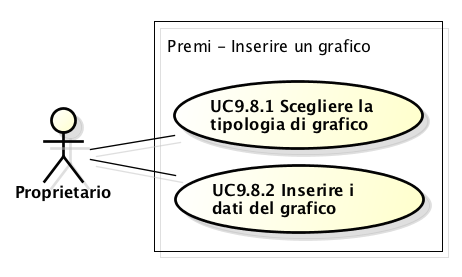
\includegraphics[scale=0.45] {img/UC9.8.png}
	\caption{UC9.8 - Inserire grafico} 
\end{figure}

\begin{itemize}
	\item \textbf{Attori:} Proprietario;
	\item \textbf{Scopo e descrizione:} L'utente deve inserire un grafico. Seleziona il tipo di grafico e inserisce i dati;
	\item \textbf{Precondizione:} Il sistema è in attesa che l'utente selezioni il comando per inserire un grafico;
	\item \textbf{Flusso principale di eventi:}
	\begin{enumerate}
		\item L'utente sceglie la tipologia di grafico da inserire [UC9.8.1];
		\item L'utente inserisce i dati da inserire nel grafico [UC9.8.2].
	\end{enumerate}
	\item \textbf{Postcondizione:} Il sistema ha creato il grafico.
\end{itemize}

	\subsection{Caso d'uso UC9.8.1: Scegliere la tipologia del grafico}
	\begin{itemize}
		\item \textbf{Attori:} Proprietario;
		\item \textbf{Scopo e descrizione:} L'utente deve scegliere il tipo di grafico da inserire;
		\item \textbf{Precondizione:} Il sistema ha aperto la finestra di dialogo per la scelta del tipo di grafico;
		\item \textbf{Postcondizione:} Il sistema ha registrato la scelta dell'utente.
	\end{itemize}
	
	\subsection{Caso d'uso UC9.8.2: Inserire i dati del grafico}
	\begin{itemize}
		\item \textbf{Attori:} Proprietario;
		\item \textbf{Scopo e descrizione:} L'utente deve inserire i dati per il grafico da inserire;
		\item \textbf{Precondizione:} Il sistema è in attesa che l'utente inserisca i dati;
		\item \textbf{Postcondizione:} Il sistema salva i dati inseriti.
	\end{itemize}


\subsection{Caso d'uso UC9.9: Scegliere un effetto di transizione}
\begin{itemize}
	\item \textbf{Attori:} Proprietario;
	\item \textbf{Scopo e descrizione:} L'utente deve scegliere l'effetto di transizione da dare alla \gls{slide};
	\item \textbf{Precondizione:} Il sistema è in attesa che l'utente selezioni l'effetto desiderato;
	\item \textbf{Postcondizione:} Il sistema ha inserito l'effetto di transizione.
\end{itemize}


\subsection{Caso d'uso UC9.10: Ridimensionamento di un elemento}
\begin{itemize}
	\item \textbf{Attori:} Proprietario;
	\item \textbf{Scopo e descrizione:} L'utente cambia la grandezza dell'elemento selezionato della \gls{slide};
	\item \textbf{Precondizione:} Il sistema mostra l'elemento selezionato che si intende ridimensionare;
	\item \textbf{Postcondizione:} Il sistema ha ridimensionato l'elemento della \gls{slide}.
\end{itemize}


\subsection{Caso d'uso UC9.11: Spostamento di un elemento}
\begin{itemize}
	\item \textbf{Attori:} Proprietario;
	\item \textbf{Scopo e descrizione:} L'utente cambia la posizione dell'elemento selezionato della \gls{slide};
	\item \textbf{Precondizione:} Il sistema mostra l'elemento selezionato che si intende spostare;
	\item \textbf{Postcondizione:} Il sistema ha spostato l'elemento della \gls{slide}.
\end{itemize}


\subsection{Caso d'uso UC9.12: Rotazione di un elemento}
\begin{itemize}
	\item \textbf{Attori:} Proprietario;
	\item \textbf{Scopo e descrizione:} L'utente ruota l'elemento selezionato della \gls{slide};
	\item \textbf{Precondizione:} Il sistema mostra l'elemento selezionato che si intende ruotare;
	\item \textbf{Postcondizione:} Il sistema ha ruotato l'elemento della \gls{slide}.
\end{itemize}


\subsection{Caso d'uso UC9.13: Rimozione di un elemento}
\begin{itemize}
	\item \textbf{Attori:} Proprietario;
	\item \textbf{Scopo e descrizione:} L'utente elimina l'elemento selezionato dalla \gls{slide};
	\item \textbf{Precondizione:} Il sistema mostra l'elemento selezionato che si intende cancellare;
	\item \textbf{Postcondizione:} Il sistema ha cancellato l'elemento dalla \gls{slide}.
\end{itemize}


\subsection{Caso d'uso UC9.14: Caricamento di un file}
\begin{itemize}
	\item \textbf{Attori:} Proprietario;
	\item \textbf{Scopo e descrizione:} L'utente deve caricare un file da utilizzare nella presentazione;
	\item \textbf{Precondizione:} Il sistema è in attesa che l'utente selezioni il file;
	\item \textbf{Postcondizione:} Il sistema ha caricato il file selezionato dall'utente e lo ha inserito nella \gls{slide}.
\end{itemize}

\newpage
\subsection{Caso d'uso UC9.15: Scegliere la formattazione del testo}
\begin{figure}[h] 
	\centering 
	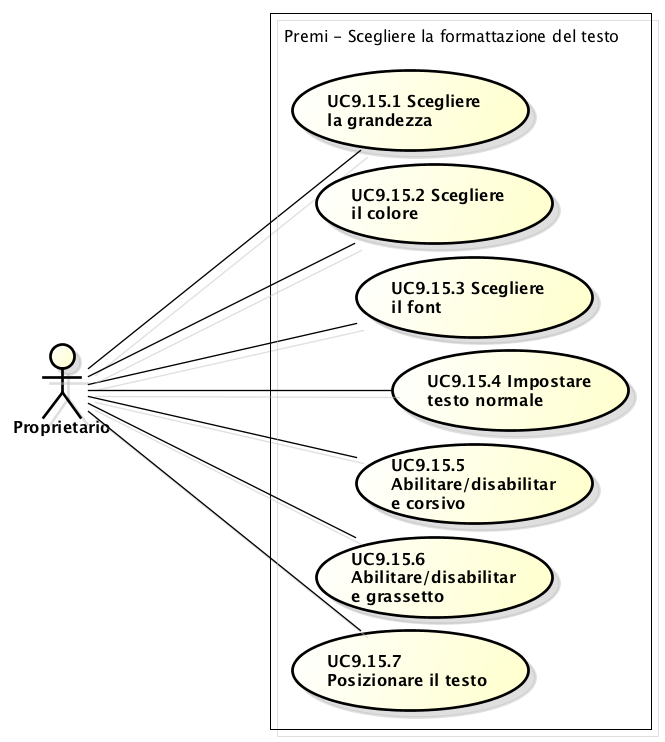
\includegraphics[scale=0.45] {img/UC9.15.png}
	\caption{UC9.15 - Scegliere la formattazione del testo}
\end{figure}

\begin{itemize}
	\item \textbf{Attori:} Proprietario;
	\item \textbf{Scopo e descrizione:} L'utente può modificare l'aspetto del testo contenuto in una casella di testo. L'utente seleziona il testo e poi sceglie che modifiche effettuare;
	\item \textbf{Precondizione:} Il sistema è in attesa che l'utente selezioni la modifica da apportare al testo e il testo da modificare è selezionato;
	\item \textbf{Flusso principale degli eventi:}
	\begin{enumerate}
		\item L'utente può cambiare la grandezza del testo [UC9.15.1];
		\item L'utente può cambiare il colore del testo [UC9.15.2];
		\item L'utente può cambiare il \gls{font} del testo [UC9.15.3];
		\item L'utente può abilitare o disabilitare il testo in corsivo [UC9.15.4];
		\item L'utente può abilitare o disabilitare il testo in grassetto [UC9.15.5];
		\item L'utente può spostare il testo in una nuova posizione [UC9.15.6].
	\end{enumerate}
	\item \textbf{Postcondizione:} Il sistema ha apportato le modifiche scelte al testo.
\end{itemize}

\subsection{Caso d'uso UC9.15.1: Scegliere la grandezza}
\begin{itemize}
	\item \textbf{Attori:} Proprietario;
	\item \textbf{Scopo e descrizione:} L'utente può cambiare la grandezza del testo;
	\item \textbf{Precondizione:} Il testo da modificare è selezionato;
	\item \textbf{Postcondizione:} Il testo è stato ingrandito o rimpicciolito secondo la scelta dell'utente.
\end{itemize}

\subsection{Caso d'uso UC9.15.2: Scegliere il colore}
\begin{itemize}
	\item \textbf{Attori:} Proprietario;
	\item \textbf{Scopo e descrizione:} L'utente può cambiare il colore del testo;
	\item \textbf{Precondizione:} Il testo da modificare è selezionato;
	\item \textbf{Postcondizione:} Il testo è stato colorato secondo la scelta dell'utente.
\end{itemize}

\subsection{Caso d'uso UC9.15.3: Scegliere il \gls{font}}
\begin{itemize}
	\item \textbf{Attori:} Proprietario;
	\item \textbf{Scopo e descrizione:} L'utente può cambiare il \gls{font} del testo;
	\item \textbf{Precondizione:} Il testo da modificare è selezionato;
	\item \textbf{Postcondizione:} Il testo ha cambiato \gls{font} secondo la scelta dell'utente.
\end{itemize}

\subsection{Caso d'uso UC9.15.4: Abilitare/disabilitare corsivo}
\begin{itemize}
	\item \textbf{Attori:} Proprietario;
	\item \textbf{Scopo e descrizione:} L'utente può abilitare o disabilitare la scrittura in corsivo;
	\item \textbf{Precondizione:} Il testo da modificare è selezionato oppure è stata selezionata la casella di testo nella quale poter scrivere;
	\item \textbf{Postcondizione:} Il testo è stato modificato secondo la scelta dell'utente.
\end{itemize}

\subsection{Caso d'uso UC9.15.5: Abilitare/Disabilitare grassetto}
\begin{itemize}
	\item \textbf{Attori:} Proprietario;
	\item \textbf{Scopo e descrizione:} L'utente può abilitare o disabilitare la scrittura in grassetto;
	\item \textbf{Precondizione:} Il testo da modificare è selezionato oppure è stata selezionata la casella di testo nella quale poter scrivere;
	\item \textbf{Postcondizione:} Il testo è stato modificato secondo la scelta dell'utente.
\end{itemize}

\subsection{Caso d'uso UC9.15.6: Posizionare il testo}
\begin{itemize}
	\item \textbf{Attori:} Proprietario;
	\item \textbf{Scopo e descrizione:} L'utente può spostare una casella di testo in una nuova posizione;
	\item \textbf{Precondizione:} La casella di testo da spostare è stata selezionata;
	\item \textbf{Postcondizione:} La casella di testo è stata spostata secondo la scelta dell'utente.
\end{itemize}

\newpage
\subsection{Caso d'uso UC9.16: Modificare una tabella}
\begin{figure}[h] 
	\centering 
	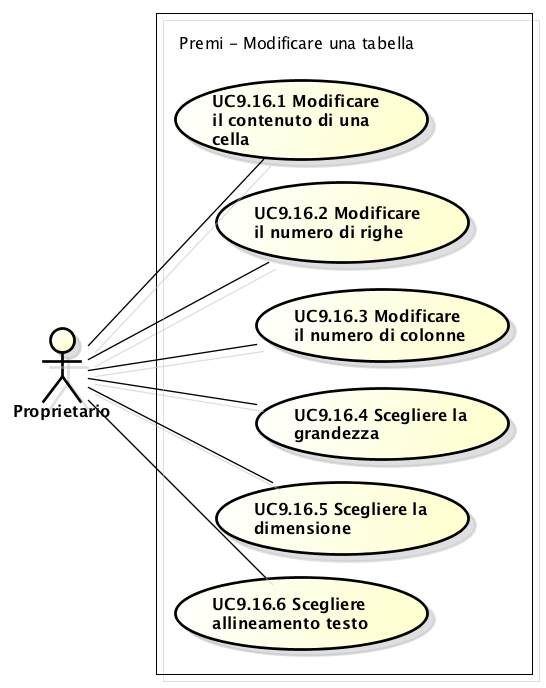
\includegraphics[scale=0.45] {img/UC9.16.png}
	\caption{UC9.16 - Modificare una tabella}
\end{figure}

\begin{itemize}
	\item \textbf{Attori:} Proprietario;
	\item \textbf{Scopo e descrizione:} L'utente può modificare l'aspetto della tabella e del suo contenuto. L'utente seleziona la tabella o il testo e poi sceglie che modifiche effettuare;
	\item \textbf{Precondizione:} Il sistema è in attesa che l'utente selezioni la modifica da apportare alla tabella e la tabella o il testo da modificare sono selezionati;
	\item \textbf{Flusso principale degli eventi:}
	\begin{enumerate}
		\item L'utente può modificare il contenuto di una cella [UC9.16.1];
		\item L'utente può modificare il numero di righe e di colonne [UC9.16.2];
		\item L'utente può cambiare la grandezza della tabella [UC9.16.3];
		\item L'utente può cambiare il colore di sfondo della tabella [UC9.16.4];
		\item L'utente può cambiare l'allineamento del testo [UC9.16.5];
		\item L'utente può cambiare la formattazione del testo [UC9.15].
	\end{enumerate}
	\item \textbf{Postcondizione:} Il sistema ha apportato le modifiche scelte alla tabella.
\end{itemize}

	\subsection{Caso d'uso UC9.16.1: Modificare il contenuto di una cella della tabella}
	\begin{itemize}
		\item \textbf{Attori:} Proprietario;
		\item \textbf{Scopo e descrizione:} L'utente può modificare il contenuto di una cella della tabella, cioè aggiungere e modificare elementi di testo;
		\item \textbf{Precondizione:} La cella da modificare è stata selezionata;
		\item \textbf{Postcondizione:} Il contenuto della cella è stato modificato.
	\end{itemize}
	
	\subsection{Caso d'uso UC9.16.2: Modificare il numero di righe e colonne della tabella}
	\begin{itemize}
		\item \textbf{Attori:} Proprietario;
		\item \textbf{Scopo e descrizione:} L'utente può modificare la grandezza della tabella;
		\item \textbf{Precondizione:} La tabella da modificare è stata selezionata;
		\item \textbf{Postcondizione:} La tabella è stata modificata nelle sue dimensioni secondo la scelta dell'utente.
	\end{itemize}
	
	\subsection{Caso d'uso UC9.16.3: Scegliere grandezza della tabella}
	\begin{itemize}
		\item \textbf{Attori:} Proprietario;
		\item \textbf{Scopo e descrizione:} L'utente può modificare la grandezza della tabella;
		\item \textbf{Precondizione:} La tabella da modificare è stata selezionata;
		\item \textbf{Postcondizione:} La tabella è stata modificata nelle sue dimensioni secondo la scelta dell'utente.
	\end{itemize}
	
	\subsection{Caso d'uso UC9.16.4: Scegliere colore di sfondo della tabella}
	\begin{itemize}
		\item \textbf{Attori:} Proprietario;
		\item \textbf{Scopo e descrizione:} L'utente può modificare il colore di sfondo della tabella;
		\item \textbf{Precondizione:} La tabella o le celle da modificare sono state selezionate;
		\item \textbf{Postcondizione:} Lo sfondo della tabella o delle celle è stato modificato secondo la scelta dell'utente.
	\end{itemize}
	
	\subsection{Caso d'uso UC9.16.5: Scegliere allineamento del testo}
	\begin{itemize}
		\item \textbf{Attori:} Proprietario;
		\item \textbf{Scopo e descrizione:} L'utente può modificare l'allineamento del testo della tabella;
		\item \textbf{Precondizione:} La tabella o le celle da modificare sono state selezionate;
		\item \textbf{Postcondizione:} L'allineamento del testo della tabella o delle celle è stato modificato secondo la scelta dell'utente.
	\end{itemize}
	
	
	\subsection{Caso d'uso UC9.17: Personalizzare un grafico}
	\begin{figure}[h] 
		\centering 
		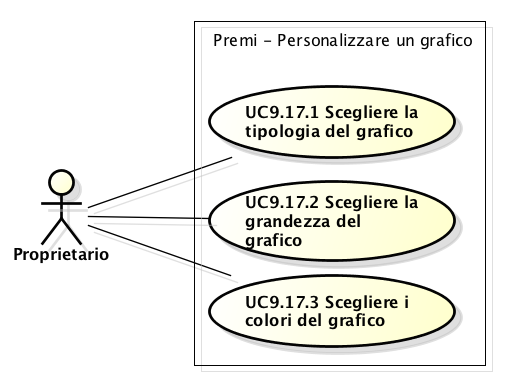
\includegraphics[scale=0.45] {img/UC9.17.png}
		\caption{UC9.17 - Personalizzare un grafico} 
	\end{figure}
	
	\begin{itemize}
		\item \textbf{Attori:} Proprietario;
		\item \textbf{Scopo e descrizione:} L'utente può modificare la tipologia e l'aspetto del grafico o del suo contenuto. L'utente seleziona il grafico e poi sceglie che modifiche effettuare;
		\item \textbf{Precondizione:} Il sistema è in attesa che l'utente selezioni la modifica da apportare al grafico e il grafico da modificare è selezionato;
		\item \textbf{Flusso principale degli eventi:}
		\begin{enumerate}
			\item L'utente può cambiare la tipologia del grafico [UC9.17.1];
			\item L'utente può cambiare la dimensione del grafico [UC9.17.2]
			\item L'utente può cambiare i colori del grafico [UC9.17.3].
		\end{enumerate}
		\item \textbf{Postcondizione:} Il sistema ha apportato le modifiche scelte al grafico.
	\end{itemize}

		\subsection{Caso d'uso UC9.17.1: Scegliere la tipologia del grafico}
		\begin{itemize}
			\item \textbf{Attori:} Proprietario;
			\item \textbf{Scopo e descrizione:} L'utente deve modificare la tipologia del grafico. Seleziona il grafico e il comando per cambiare il tipo;
			\item \textbf{Precondizione:} Il grafico da modificare è stata selezionato e il sistema è in attesa che l'utente selezioni il comando;
			\item \textbf{Postcondizione:} La tipologia del grafico è stata modificata secondo la scelta dell'utente.
		\end{itemize}
		
		\subsection{Caso d'uso UC9.17.2: Scegliere la grandezza del grafico}
		\begin{itemize}
			\item \textbf{Attori:} Proprietario;
			\item \textbf{Scopo e descrizione:} L'utente deve modificare la grandezza del grafico;
			\item \textbf{Precondizione:} Il grafico da modificare è stato selezionato;
			\item \textbf{Postcondizione:} Il grafico è stato modificato nelle sue dimensioni secondo la scelta dell'utente.
		\end{itemize}
		
		\subsection{Caso d'uso UC9.17.3: Scegliere i colori del grafico}
		\begin{itemize}
			\item \textbf{Attori:} Proprietario;
			\item \textbf{Scopo e descrizione:} L'utente deve modificare il set di colori del grafico;
			\item \textbf{Precondizione:} Il grafico da modificare è stato selezionato e il sistema è in attesa che l'utente selezioni il comando;
			\item \textbf{Postcondizione:} I colori del grafico sono stati modificati secondo la scelta dell'utente.
		\end{itemize}


\subsection{Caso d'uso UC9.18: Inserire note / parole chiave}
\begin{itemize}
	\item \textbf{Attori:} Proprietario;
	\item \textbf{Scopo e descrizione:} L'utente deve inserire delle note o delle parole chiave nella \gls{slide} da usare durante la visualizzazione della presentazione in modalità presentatore. Seleziona il comando e inserisce ciò che desidera includere;
	\item \textbf{Precondizione:} Il sistema è in attesa che venga selezionato il comando per inserire una nota/parola chiave;
	\item \textbf{Postcondizione:} Il sistema inserisce le note/parole chiave che l'utente ha aggiunto.
\end{itemize}

